
\lfoot{Autor: Fitim Faiku}
\subsubsection{Grundsätze einer Android Applikation}
\label{subsec:aapp-fundam}

Android Apps werden in der Programmiersprache Java geschrieben.
Die Android SDK-Tools kompilieren Code zusammen mit allen Ressourcen-Dateien in eine APK.
Eine APK ist ein Android-Paket, welches alle Inhalte einer Android App enthält. 
Die APK-Datei wird dann auf das Android-Gerät installiert. 


\textbf{Native vs HTML5 vs Hybrid} \newline
Bei der Umsetzung unserer Android Applikation, war die Entscheidung, wie wir die Android App erstellen. 
Da Android mehrere Programmierarten unterstützt wurde evaluiert welche Programmiermodule für unsere App am besten geeignet sind. \nextline

\textbf{Native\newline} 
Der Vorteil an Native Apps ist, das sie auf die Hardware wie z.B. Kamera und GPS Sensoren zugriff haben. 
Weiterhin ist der Verkauf nicht sehr schwer, da es auf dem Play-Store vertrieben werden kann. 
Für native Apps wird auf der Android-Plattform die Programmiersprache Java verwendet.
Native Apps zeigen die beste Performance.
Die Dokumentation zu Nativen Apps ist am besten, da es über 2500 Bücher zur Android Entwicklung gibt.
Für nativ Apps werden Entwicklungsumgebungen-IDE(Integrated Developement Enviroment) verwendet um die gewünschte App zu Programmieren.
Es wurde Android Studio als IDE verwendet, welche als einzige von Google unterstützt wird.
\nextline


\textbf{HTML5\newline} 
Da eine HTML 5 Applikation über den Webbrowser verwendet wird, sind die Entwickler nicht von anderen Plattformen abhängig. 
HTML5 verwendet Standard Web Technologien, wie JavaScript und CSS.
HTML5 Applikationen werden über Browser benutzt, wobei jedes Gerät auf einem Browser zugreifen kann und dadurch die App auf allen mobilen Plattformen abgespielt werden kann. \nextline

\textbf{Hybrid\newline} 
Hybrid Apps sind eine Mischung aus nativ und HTML5 Apps. Hybrid bietet den besten Kompromiss. Das Design wird mittels HTML5 und CSS erstellt, wobei sich dahinter ein JavaScript-Code befindet. Hybrid Apps sind genauso auf jeder Plattform abspielbar, wobei sie für die verschiedenen Plattformen entsprechend umprogrammiert werden müssten. 
\cite{Faik.CH2-app-fundam_Vergleich} 
\clearpage

\subsubsection{Android Virtual Device}
Ein Android Virtual Device(AVD) ist eine Emulator-Konfiguration, welche benutzt werden kann, um die entwickelte App darzustellen. 
Der einfachste Weg, um ein AVD zu schaffen, ist, den AVD-Manager in Android-Studio zu nutzen. 
Es kann auch auf performantere AVDs zurückgegriffen werden, um damit optimierte Applikationen zu schreiben.
Diese externen AVDs bieten eine realitätsnahe Darstellung des verwendeten Devices.
Für die Verwenden der AVD müssen System-image Packages herunter geladen werden, wodurch die Software der AVD zugeordnet wird und mit verschiedenen API Versionen gearbeitet werden kann.
Eine API(Application Programming Interface) ist die Version der Programmierstelle, wobei aktuellere Feauters auf höheren Versionen möglich sind. 
Eine Zuordnung zu einem System-Image: Es kann festlegen werden, welche Version der Android-Plattform auf dem virtuellen Gerät ausgeführt werden. Es kann eine Version der Standard-Android-Plattform oder System-Image mit einem SDK Add-on verpackt wählen.

Es können so viele verschiedene AVDs erstellt werden, basierend auf den Devicetypen mit denen man arbeiten möchte.
Folgende Punkte sollten beachtet werden, wenn System-image für die AVD ausgewählt werden:
Der API Level für das Device ist wichtig, da einige Applikationen auf niedrigeren API Level nicht lauffähig sind. Beim Verwenden von libraries muss beachtet werden ab welche API Version die Library verfügbar ist, da das Arbeiten mit falschem API-Level nicht möglich ist.


\begin{figure}[!tbp]
	\centering
	\begin{minipage}[b]{0.4\textwidth}
		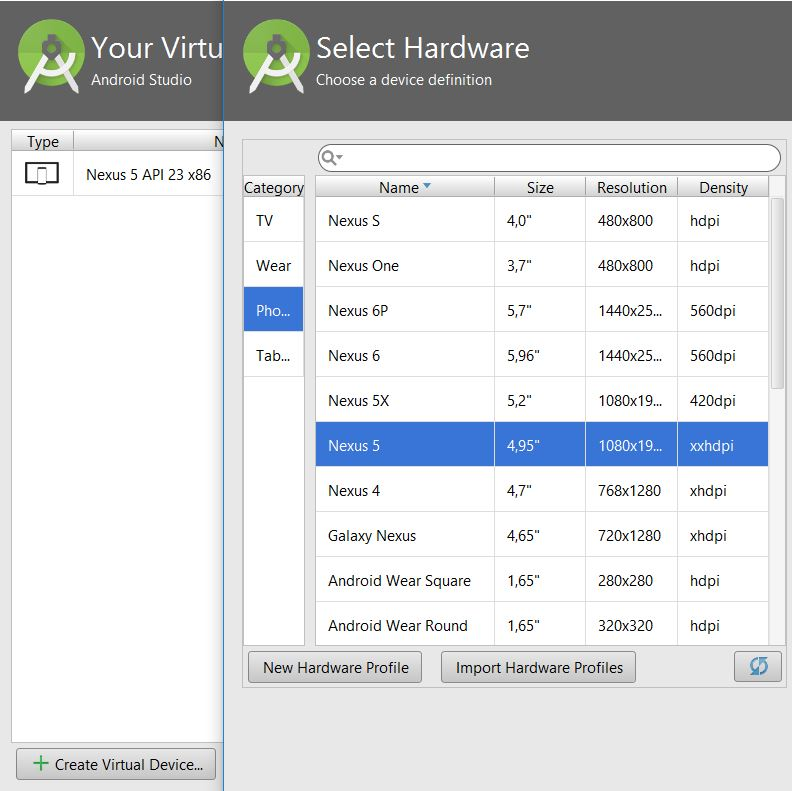
\includegraphics[width=\textwidth]{images/Create-virtual-device.jpg}
		\caption{Erstellen einer AVD in Android Studio}
	\end{minipage}
	\hfill
	\begin{minipage}[b]{0.4\textwidth}
		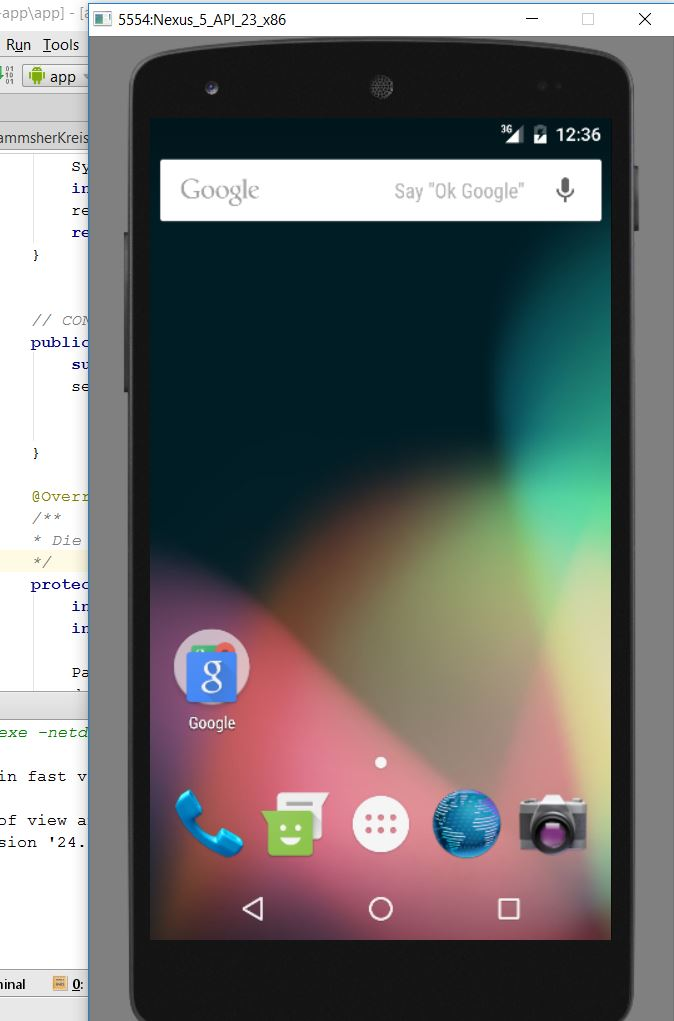
\includegraphics[width=\textwidth]{images/AVD.jpg}
		\caption{Android Virtual Device}
	\end{minipage}
\end{figure}


\clearpage % DO NOT REMOVE